\documentclass[liststotoc,bibtotoc,fontsize=14pt,]{scrreprt}
\usepackage[utf8]{inputenc} % Zeichenkodierung
\usepackage[ngerman]{babel} % neue deutsche Rechtschreibung
\usepackage{etoolbox}
\setlength{\footskip}{30pt}
\apptocmd{\thebibliography}{\raggedright}{}{}
\usepackage{graphicx}
\usepackage{caption}
\usepackage{subcaption}
\usepackage{url}
\usepackage[onehalfspacing]{setspace}
\usepackage{breakurl}
\usepackage{float}
\usepackage[table,xcdraw]{xcolor}
\usepackage{tabularx}
\usepackage[breaklinks]{hyperref}
\def\UrlBreaks{\do\/\do-}
\usepackage{tocloft}
\usepackage{chngcntr}
\usepackage{listings}
\usepackage{color}
\usepackage[parfill]{parskip}
\definecolor{lightgray}{rgb}{.9,.9,.9}
\definecolor{darkgray}{rgb}{.4,.4,.4} 
\definecolor{purple}{rgb}{0.65, 0.12, 0.82}

\counterwithout{footnote}{chapter}

\deffootnote[2em]{2em}{2em}{%
	\makebox[2em][l]{\bfseries\thefootnotemark}}

\renewcommand{\cftchapdotsep}{\cftdotsep}
\renewcommand{\cftchapleader}{\cftdotfill{\cftchapdotsep}}
\usepackage{amsmath}
\usepackage[paper=a4paper,left=30mm,right=30mm,top=25mm,bottom=25mm]{geometry}
\usepackage[section]{placeins}
\usepackage[font=small,justification=justified]{caption}
\newcommand{\namesigdate}[3][Ort, Datum]{%
	\parbox{\textwidth}{
		\raggedleft #3 
		\vspace{2cm}
		
		\parbox{5cm}{
			\raggedright
			\rule{6cm}{1pt}\\
			#1 
		}
		\hfill
		\parbox{5cm}{
			\raggedright
			\rule{6cm}{1pt}\\
			#2
		}
	}
}


\newcommand*{\tabularwidth}{}
\newdimen\tabularwidth
\usepackage{minitoc}
\hypersetup{
	colorlinks,
	citecolor=black,
	filecolor=black,
	linkcolor=black,
	urlcolor=black
}


\title{Dokumentation Stereo-Fotografie}
\author{Sebastian Degner}

\begin{document}
	%\maketitle
	
	\begin{titlepage}
		\begin{center}
			\vspace{2cm}
			Dokumentation\\ \textbf{Multishot-Technik in der digitalen Fotografie}\\ 
			\vspace{2,5cm}
			
\includegraphics[width=5cm]{HTWK_Logo_RGB-transparent_250.png}\\
			
			\vspace{2,5cm}
			\huge \textbf{\textsf{Dokumentation Stereo-Fotografie}} \\
			\vspace{3cm}
			\fontsize{15}{18} \textbf{Hochschule für Technik, Wirtschaft und Kultur
				Leipzig\\ Fakultät Informatik, Mathematik und Naturwissenschaften\\   Masterstudiengang Medieninformatik}\\
			\vspace{3cm}
		\end{center}
		\normalsize{
			\begin{tabular}{ll}
				Eingereicht von: & {Sebastian Degner} \\
				 & {Sebastian Knabe} \\
				Studiengang: & 15 MIM\\
				Eingereicht am: & 03. März 2017 \\
			\end{tabular}\\
		}
		
	\end{titlepage}
	
	\tableofcontents
	\clearpage
	\listoffigures
	\addcontentsline{toc}{chapter}{Abbildungsverzeichnis}

	\chapter{Einleitung}
	\label{ch:einleitung}
	Im Rahmen des \textit{Moduls Multishot-Technik in der digitalen Fotografie} wurde diese Dokumentation zu dem Thema \textit{High Dynamic Range} (auch mit HDR abgekürzt) realisiert. Mit Hilfe der HDR-Fotografie lassen sich Aufnahmen erstellen, die einen besonders hohen Kontrastumfang aufweisen. Fotos, welche mit dieser Technik aufgenommen werden, können Helligkeitsunterschiede detailreich wiedergeben. Außerdem wird vermieden, dass Bildinformation durch Über- beziehungsweise Unterbelichtung verloren gehen. HDR-Aufnahmen können mit  einer handelsüblichen Spiegelreflexkamera nicht direkt aufgenommen werden. Um diese zu erzeugen, muss man mehrere Einzelbilder aufnehmen, welche später mit Hilfe spezieller Software zu einem HDR-Foto zusammengefügt werden.
	
			
	\chapter{Aufnahmen}
	\label{ch:aufnahmen}
	
	\section{Paulinum }
	\label{sec:spinnerei}

	\subsubsection{Aufnahmeort und -idee}

		\begin{figure}[H]
			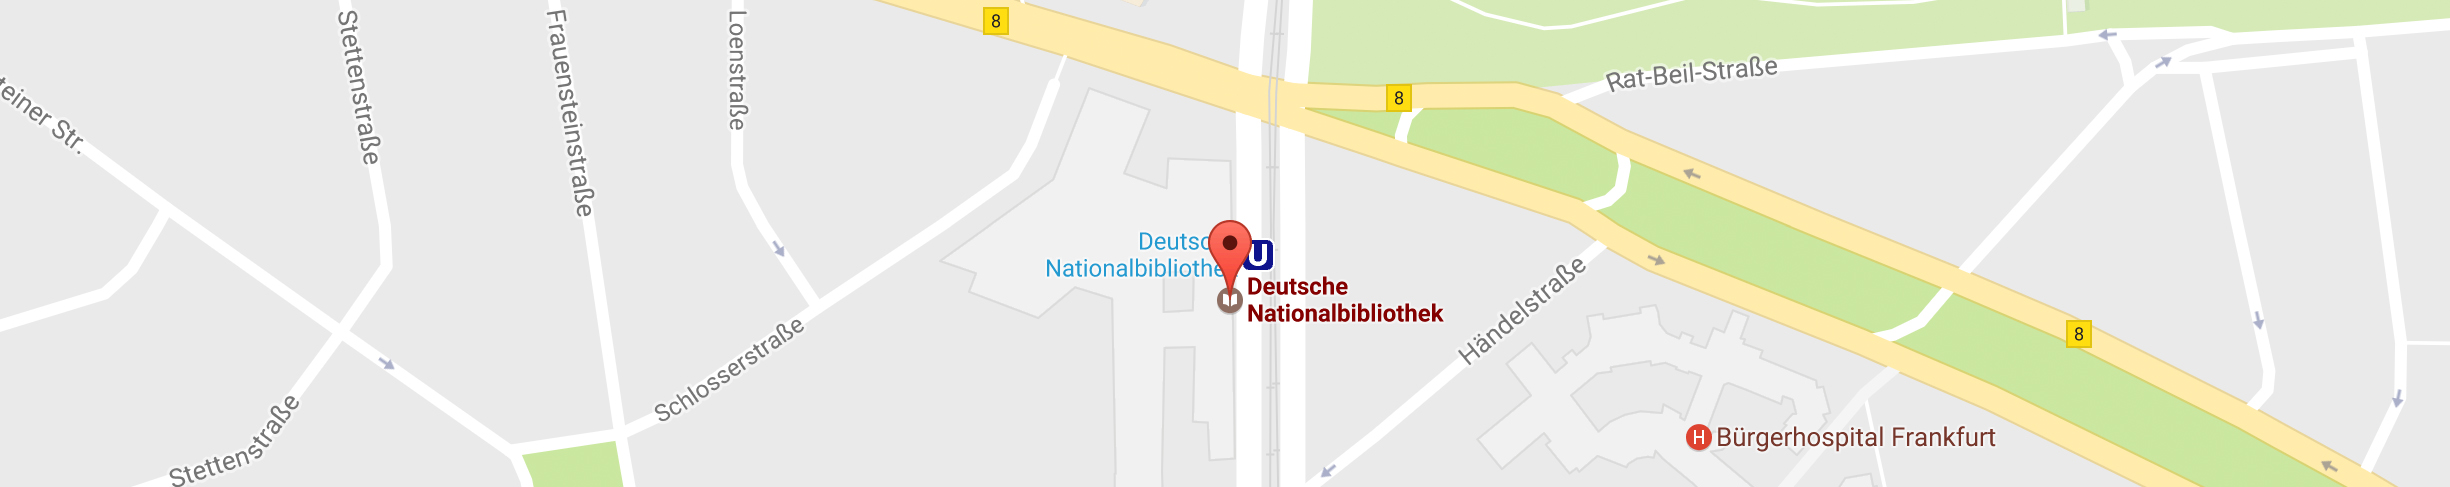
\includegraphics[width=\linewidth]{img/places/bibo_map.jpg}
			\caption{Aufnahmeort Paulinum}
			\label{img:paulinum_map}
		\end{figure}

		\subsubsection{Kameraeinstellungen}
			\begin{minipage}{0.58\textwidth}
				\begin{tabular}{ll}
					Kamera: &Canon EOS 7D \\
					Objektiv: &Canon EF 10-22mm \\
					& F/3.5-4.5 USM\\		
					Brennweite:& 10mm \\
					Belichtungszeit: & $\frac{1}{30}$s /$\frac{1}{15}$s /$\frac{1}{4}$s / $\frac{1}{2}$s \\
					 & 1s\\
					Blendenwert: & f/8\\
					Empfindlichkeit & ISO 100 \\
				\end{tabular}\\
			\end{minipage}%
			\begin{minipage}{0.42\textwidth}
				\begin{figure}[H]
					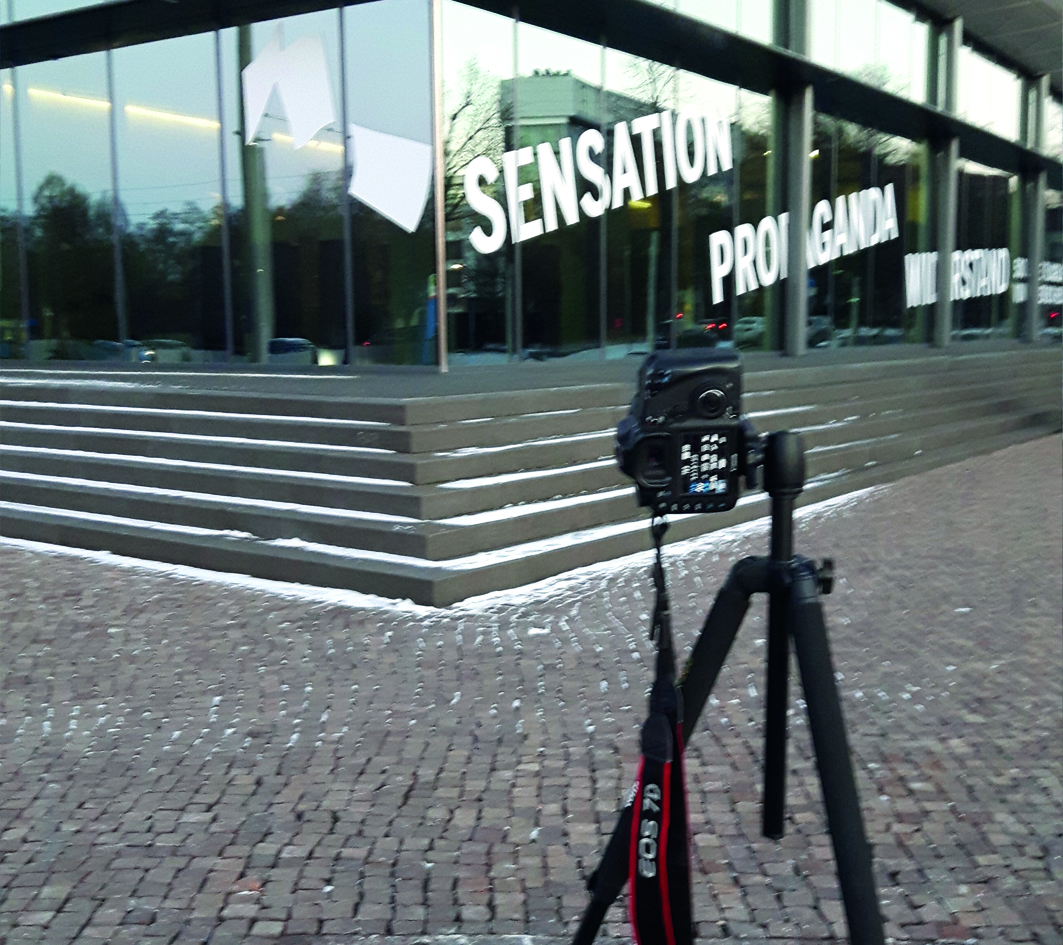
\includegraphics[width=\linewidth]{img/places/bibo.jpg}
					\caption{Aufnahmesituation Paulinum}
					\label{img:ak}
				\end{figure}
			\end{minipage}%

	\subsubsection{Vorgehen}

	
	\newpage
	\begin{figure}[h]
		
\includegraphics[width=\linewidth]{img/ph.jpg}
		\caption{Stereo-Aufnahme Paulinum}
	\end{figure}

\section{Karl-Heine-Denkmal}
\label{sec:palme}
\subsubsection{Aufnahmeort und -idee}



\subsubsection{Vorgehen}

\newpage
\begin{figure}[h]
	
\includegraphics[width=\linewidth]{img/ph.jpg}
	\caption{Stereo-Aufnahme Karl-Heine-Denkmal}
\end{figure}

\section{Leipziger Österreicher-Denkmal}
\label{sec:nikolai}
\subsubsection{Aufnahmeort und -idee}


\subsubsection{Vorgehen}


\newpage
\begin{figure}[h]
	
\includegraphics[width=\linewidth]{img/ph.jpg}
	\caption{Stereo-Aufnahme Österreicher-Denkmal}
\end{figure}
	
	\section{Richard-Wagner-Platz}
	\label{sec:tunnel}
	\subsubsection{Aufnahmeort und -idee}
		
	\subsubsection{Vorgehen}


			 \newpage
			 \begin{figure}[h]
			 	
\includegraphics[width=\linewidth]{img/ph.jpg}
			 	\caption{Stereo-Aufnahme Richard-Wagner-Platz}
			 \end{figure}




	\chapter{Vorbereitung}
	
	
	\section{Einzelbildaufnahmen}
	 

	\chapter{Stereo-Erstellung}

	

	
	\chapter{Nachbearbeitung}

	
\end{document}